\chapter{Formal analysis using Alloy}
	\paragraph{}
		In this section, the system is described using an Alloy model.
		The model contains all entities involved in the system and their attributes, following the schema given by the class diagram.
		Some relations between entities are highlighted and expressed as static constraints:
		\begin{itemize}
			\item It cannot happen that two different registered entities have the same username or that an email address is associated with more than one account
			\item Each position must belong to one and only one municipality and if a position is the center of a municipality it must belong to that municipality
			\item It cannot happen that a user, a vehicle, a ticket or an accident are registered in different positions at the same time
			\item If a valid report or an accident occurred on a position, there must be at least one improvement suggestion for that position, but there must not be suggestion without having problems on a position
			\item If the plate of the vehicle in a report is not recognized by the OCRS, the report must be set as "Not valid", but there can be reports set as "Not valid" with a valid license plate recognized
			\item Each municipality can access only to reports occurred on its territory
			\item Each RU can access only to his/her reports
		\end{itemize}
		
		Then, some other necessary structural constraints are expressed and properly commented in the Alloy formal notation. These are verified analyzing the worlds generated running the model.
		It is also highlighted how the addition of a report involves the municipality, the user, the vehicle and the position.
		\clearpage
		\section{World model}
			\lstinputlisting[language=alloy]{alloy/Alloy.als}
			\begin{figure}[!h]
						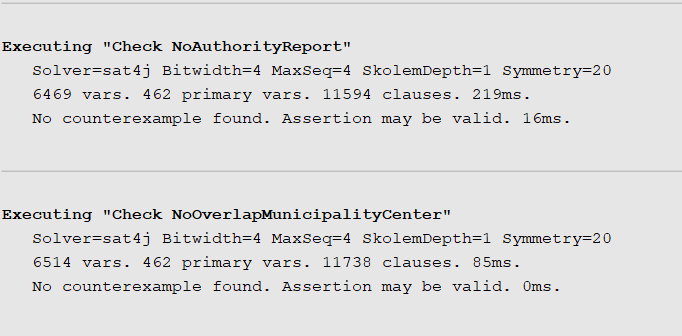
\includegraphics[width=\textwidth]{images/Alloy/Assert.png}
						\caption{Alloy assert execution}
					\end{figure}
					\begin{figure}[!h]
						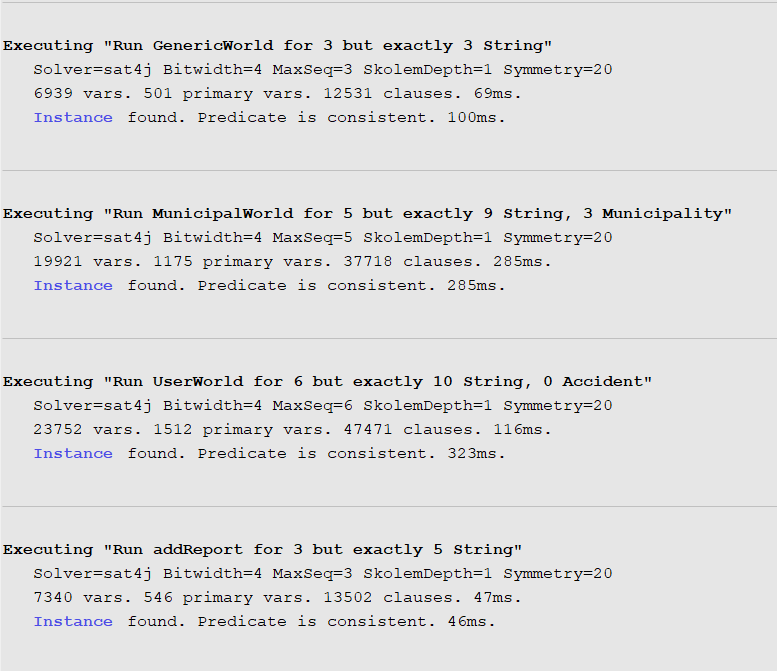
\includegraphics[width=\textwidth]{images/Alloy/Worlds.png}
						\caption{Alloy worlds execution}
					\end{figure}
		\section{Generated world}
			\subsection{Generic world}
				\paragraph{}
					This is an example of a generic world, with entities and their relations.
					
					Each position belongs to only one municipality (which center position belongs to it too) and they don't share reports. 
					
					A user can send reports to different municipalities and can access only to all his/her past reports.
					
					Authorities are not related to reports.
					
					Improvements are generated if and only if a problem occurred in a certain position.
					
					There are no ubiquity problems.
					\begin{figure}[!h]
						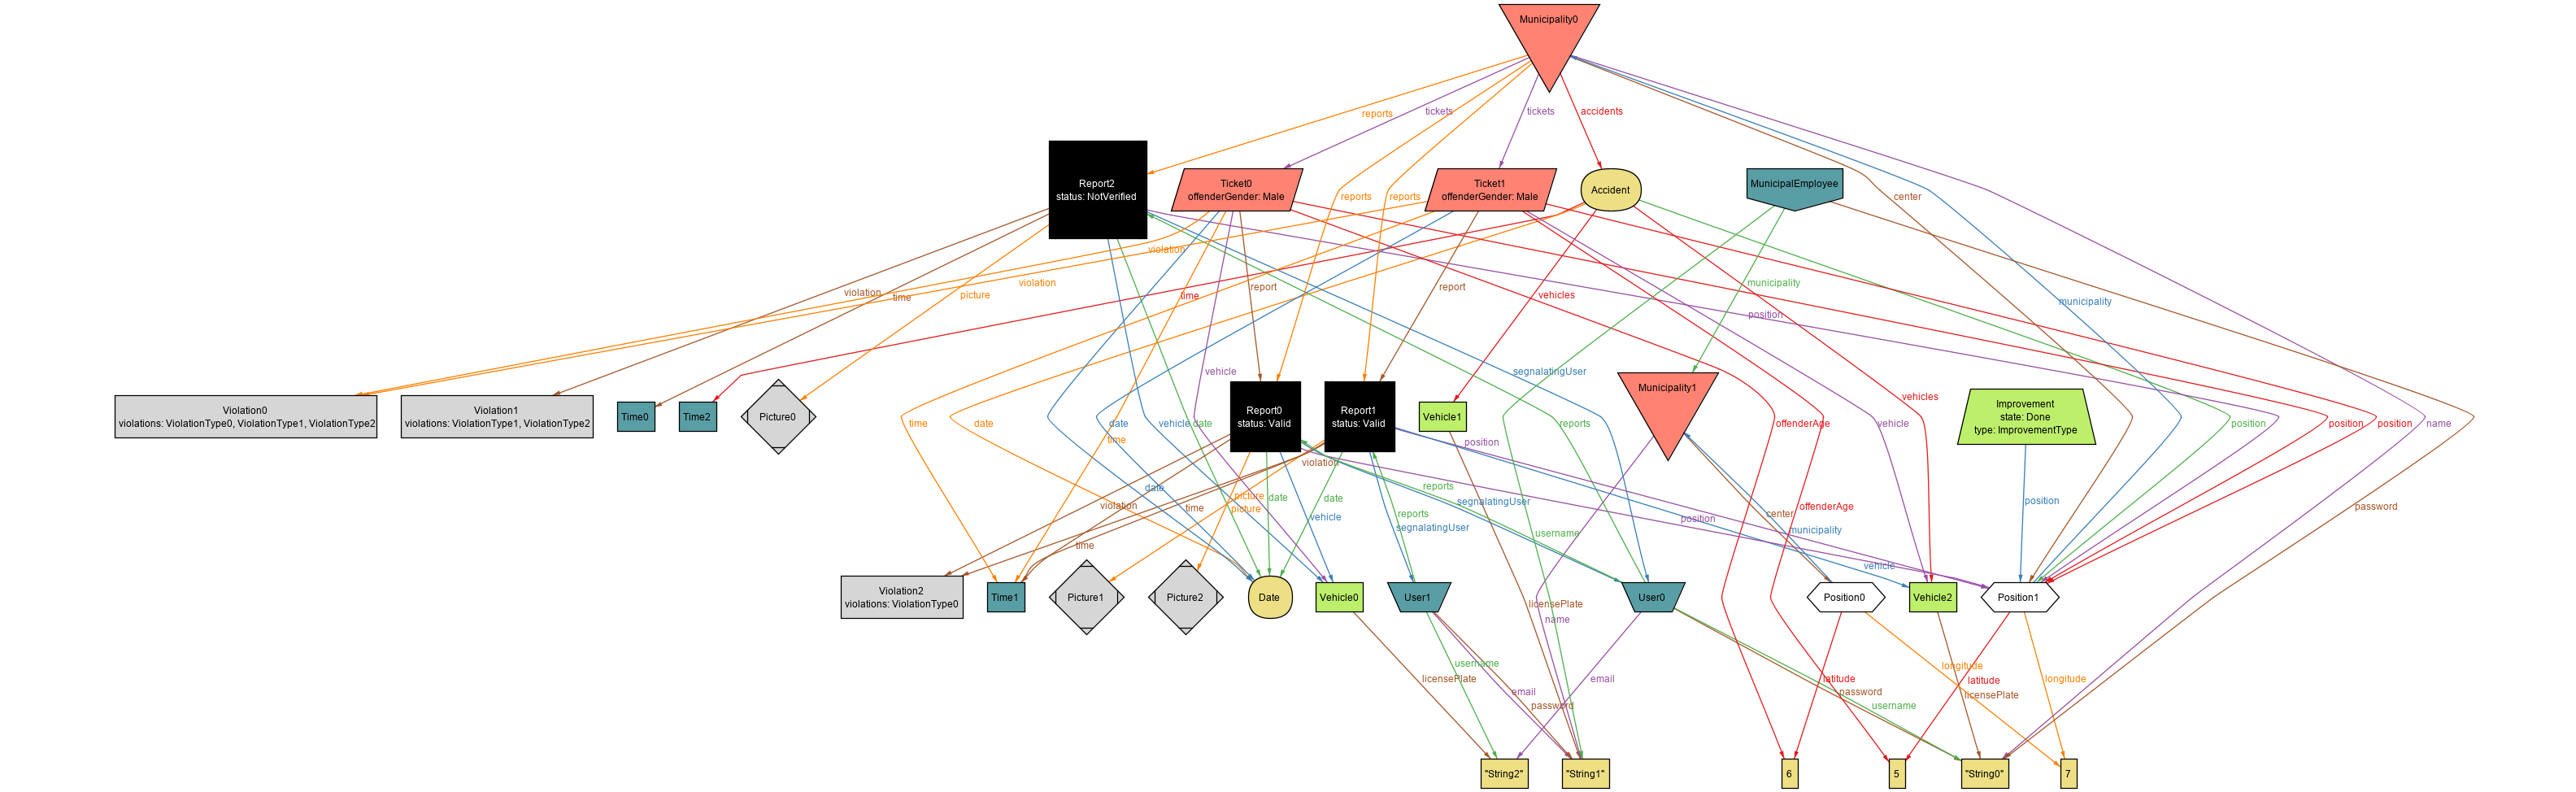
\includegraphics[width=\textwidth]{images/Alloy/GenericWorld.png}
						\caption{Alloy generic world}
					\end{figure}
			\subsubsection{Municipal world}
				\paragraph{}
					This world highlights the associations occurring into a municipality, such as received reports, issued tickets, occurred accidents and suggested improvements. It also shows how positions are related to municipalities and what occurred on them.
					
					Each municipality can access only to reports that occurred on its territory. It can also get improvements only in positions belonging to its territory.
					\begin{figure}[!h]
						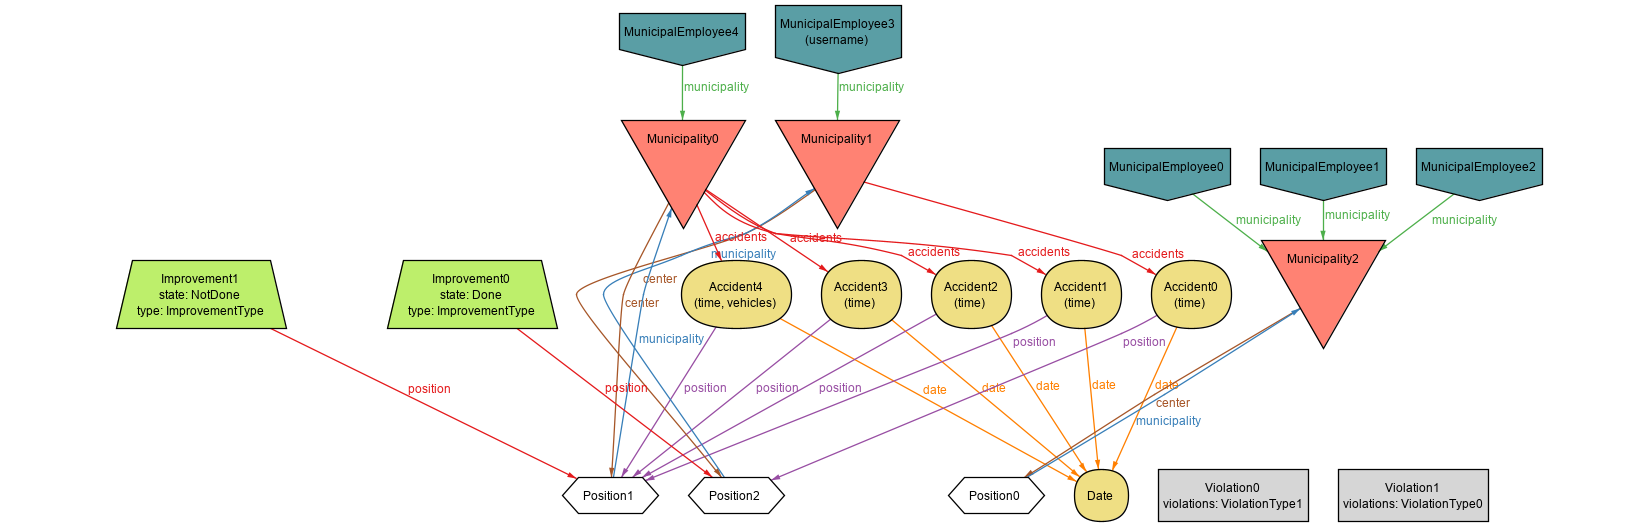
\includegraphics[width=\textwidth]{images/Alloy/MunicipalWorld.png}
						\caption{Alloy municipal world}
					\end{figure}
			\clearpage
			\subsubsection{User world}
				\paragraph{}
					This world highlights the associations between users and reports.
					
					Each user can access only to his/her past reports, whatever the municipality on which each one occurred.
					\begin{figure}[!h]
						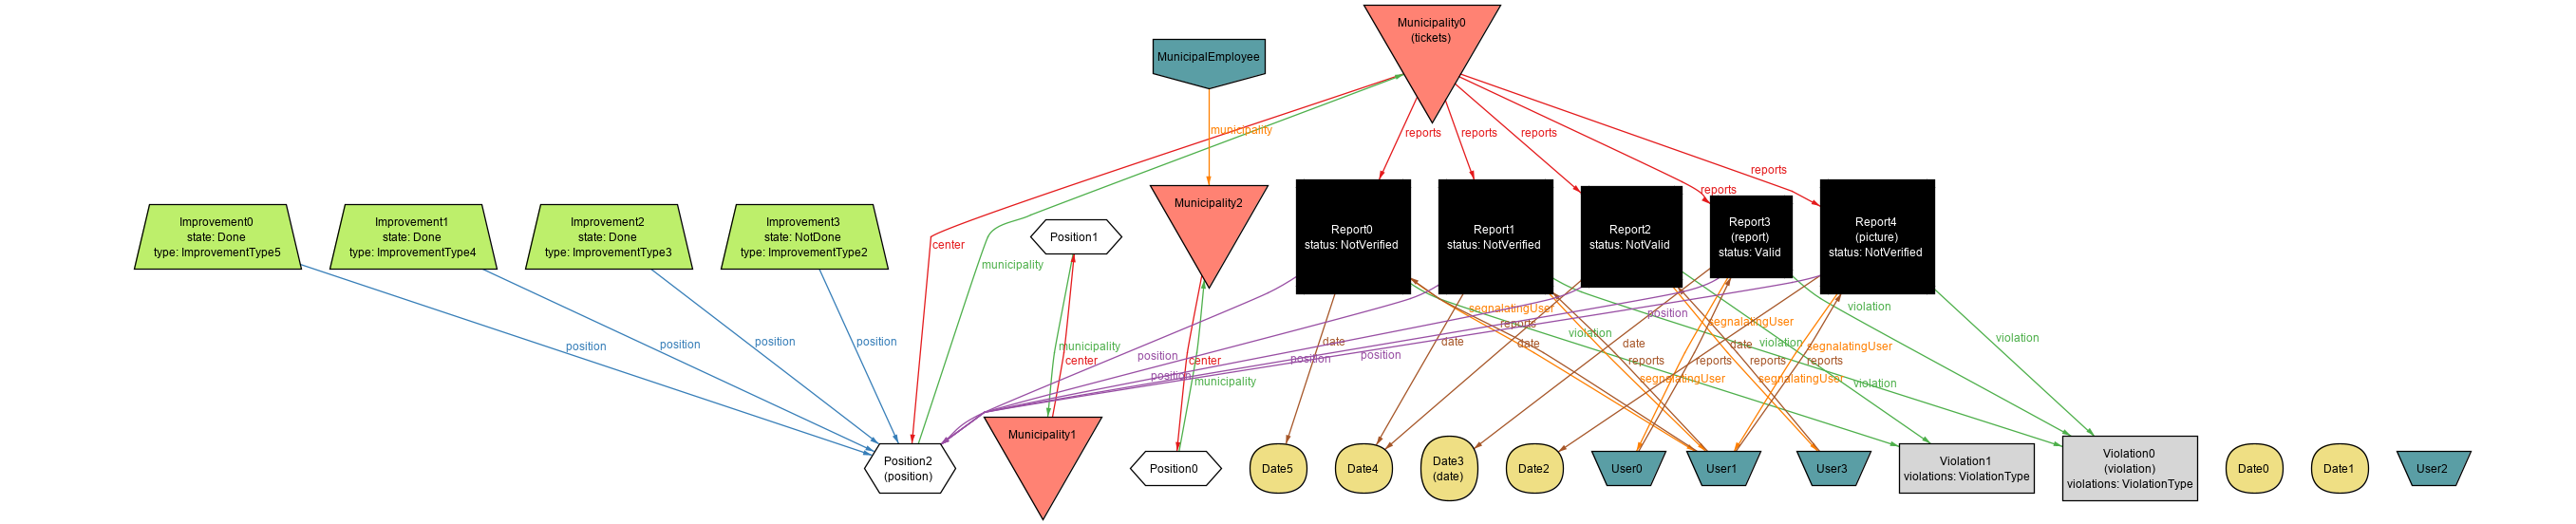
\includegraphics[width=\textwidth]{images/Alloy/UserWorld.png}
						\caption{Alloy user world}
					\end{figure}
			\subsubsection{Add report}
				\paragraph{}
					It shows how an "add report" event occurred, being related to user and municipality, and also to the vehicle and the position, eventually making possible the generation of a possible improvement if the report is valid.
					\begin{figure}[!h]
						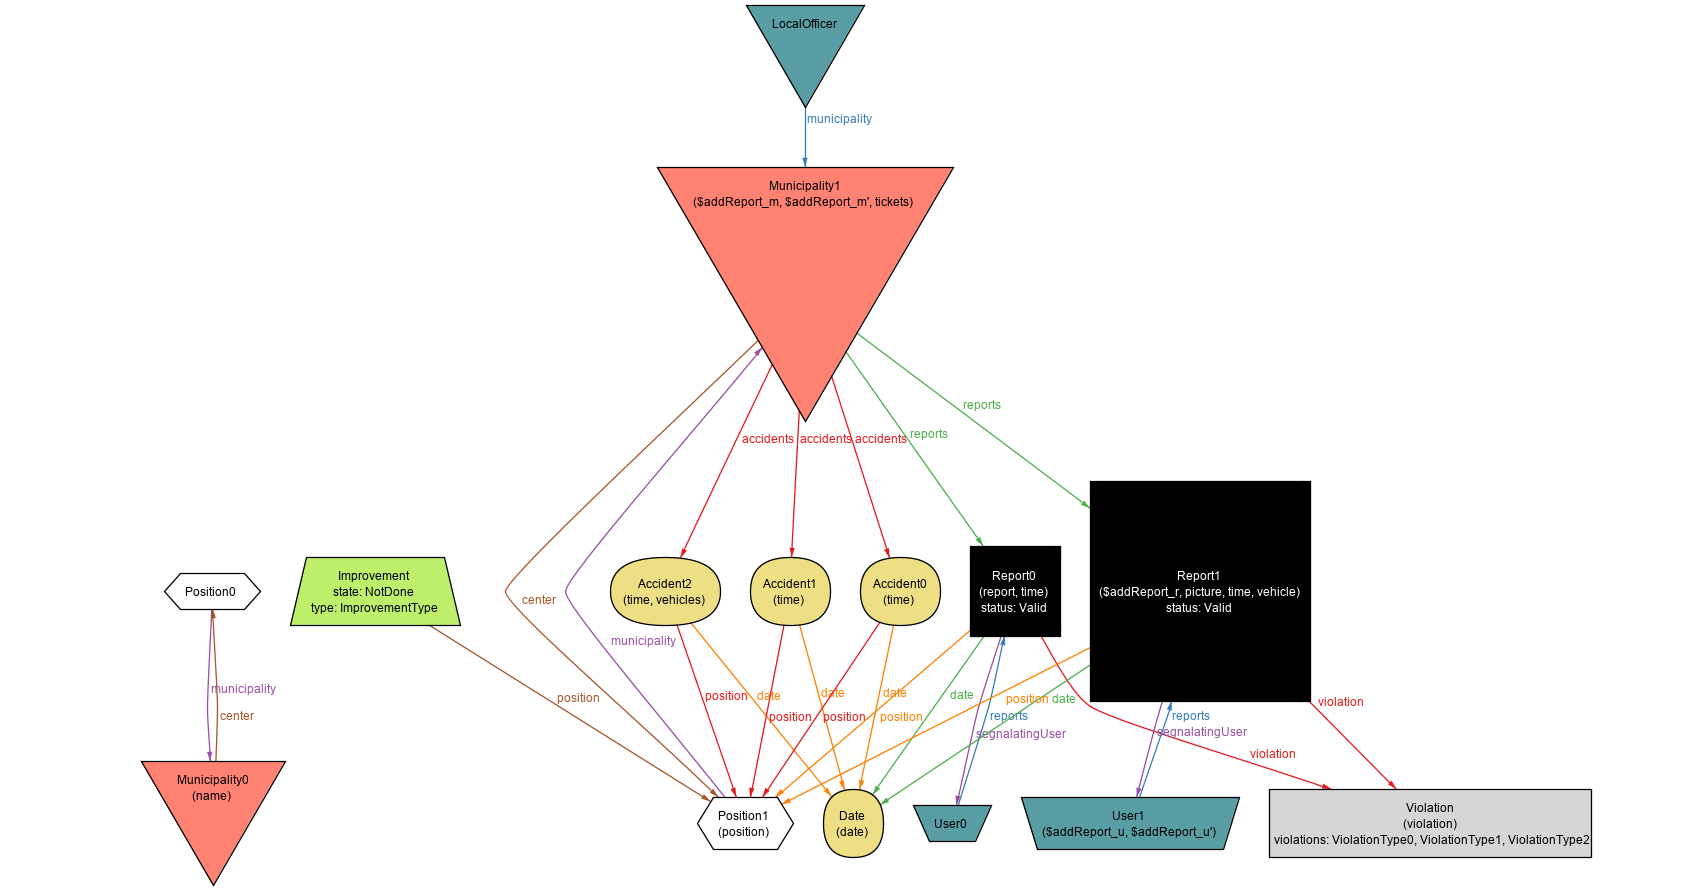
\includegraphics[width=\textwidth]{images/Alloy/AddReport.png}
						\caption{Alloy add report}
					\end{figure}
	